\documentclass[A4,12PT, english, twocolumn]{journal}
\usepackage{amsmath,amssymb,amsfonts}
\usepackage[margin=0.7in]{geometry}
\usepackage{graphicx}
\usepackage{enumitem}
\usepackage{xcolor}
\usepackage{hyperref}
\usepackage{tabularray}
\usepackage{multicol}
\usepackage{tikz}
\usepackage{circuitikz}
\usepackage{scalerel}
\usepackage{pict2e}
\usepackage{tkz-euclide}
\usetikzlibrary{calc}
\usetikzlibrary{patterns,arrows.meta}
\usetikzlibrary{shadows}
\usetikzlibrary{external}

%pgfplots
\usepackage{pgfplots}
\pgfplotsset{compat=newest}
\usepgfplotslibrary{statistics}
\usepgfplotslibrary{fillbetween}

\def\infinity{\rotatebox{90}{8}}

% Hiperlink
\hypersetup{
    colorlinks=true,
    linkcolor=blue,
    filecolor=magenta,      
    urlcolor=cyan,
    pdftitle={Overleaf Example},
    pdfpagemode=FullScreen,
}
%\usepackage{style}
\NewDocumentCommand{\Log}{o}{%
\IfNoValueTF{#1}{}{{}^{#1}\!}\log}%
  
%command buat logaritma dengan basisnya di pojok kiri
%\textheight=17cm
%\textwidth=10cm
%\usepackage{blindtext}
\setenumerate[1]{itemsep=0,5cm}
\setenumerate[2]{topsep=5pt, itemsep=5pt, label=\textbf{\Alph*}.}

\title{Matematika Saintek \& Fisika UTUL UGM 2015 Kode 632}
\author{Fauzan Akbar Sukandar Putra \\ \LaTeX}

\begin{document}

\maketitle

%\begin{minipage}{0.5\textwidth}
\begin{enumerate}
% DIAMBIL SECARA RANDOM DARI BERBAGAI SUMBER%

%1%
\item Hasil pencerminan titik $C(-4,-2)$ terhadap garis \\ $ax+by+6=0$ adalah $C'(4,10)$. Nilai $a+2b$ adalah\dots
    \begin{enumerate}
        \item $-8$.
        \item $-4$.
        \item $2$.
        \item $4$.
        \item $8$.
    \end{enumerate}
  
%2%
\item Nilai minimum fungsi $f(x)=2\sin x+\cos 2x$ pada \\ $0\le x\le 2\pi$ adalah\dots
    \begin{enumerate}
        \item $-4$.
        \item $-3$.
        \item $-2$.
        \item $-1$.
        \item $0$.
    \end{enumerate}
     
%3%
\item Jika garis $2x+y+4=0$ dan $2x+y-6=0$ menyinggung lingkaran dengan pusat $(1,p)$ Maka persamaan lingkaran tersebut adalah\dots
    \begin{enumerate}
        \item $x^2+y^2-2x+2y-3=0$.
        \item $x^2+y^2-2x-2y-3=0$.
        \item $x^2+y^2-2x+4y-3=0$.
        \item $x^2+y^2-2x-4y-3=0$.
        \item $x^2+y^2-2x+4y=0$.
    \end{enumerate}

%4%
\item Diketahui kubus $ABCD.EFGH$ dengan panjang rusuk $4p$. Titik $P, \; Q,$ dan $R$ berturut-turut terletak pada rusuk $FG, \; BF,$ dan $GH$ dengan $GP = BQ = GR = p$. Sudut antara bidang yang melalui titik $P, \; Q, \; R$ dan bidang $ABCD$ adalah $\alpha$. Nilai $\tan{\alpha}$ adalah\dots
    \begin{enumerate}
        \item $\frac{\sqrt{2}}{2}$.
        \item $\frac{\sqrt{3}}{2}$.
        \item $1$.
        \item $\sqrt{2}$.
        \item $\sqrt{3}$.
    \end{enumerate}

%5%
\item Diketahui vektor $\vec{p}=\hat{i}+2\hat{j}+c\hat{k}$, $\vec{q}=\hat{i}+2\hat{j}+c\hat{k}$, dan $\vec{r}=3\hat{i}+6\hat{j}+c\hat{k}$ dengan $a, \; b\ne 0$. Jika $p\bot q$ dan $p\bot r$, maka $\frac{{{a}^{2}}+4{{b}^{2}}}{ab}=$\dots
    \begin{enumerate}
        \item $-8$.
        \item $-4$.
        \item $-2$.
        \item $2$.
        \item $4$.
    \end{enumerate}

%6%
\item Jika $x_1$ dan $x_2$ memenuhi $|3x-4|=x+5$, maka nilai $x_1+x_2$ adalah\dots
    \begin{enumerate}
        \item $\frac{13}{4}$.
        \item $\frac{15}{4}$.
        \item $\frac{17}{4}$.
        \item $\frac{19}{4}$.
        \item $\frac{21}{4}$.
    \end{enumerate}

%7%
\item Jika $9, \; x_1$, dan $x_2$ merupakan tiga akar berbeda dari \\ $x^3-6x^2-ax+b=0$ dengan $b-a=5$, maka \\ $x_1+x_2+x_1.x_2=$\dots
    \begin{enumerate}
        \item $-7$.
        \item $-4$.
        \item $-1$.
        \item $1$.
        \item $3$.
    \end{enumerate}

%8%
\item Pertidaksamaan ${{(3x)}^{1+{}^{3}\log 3x}} > 81{{x}^{2}}$ mempunyai penyelesaian\dots
    \begin{enumerate}
        \item $x > 3$.
        \item $x < \frac{1}{9}$.
        \item $x < \frac{1}{3}$.
        \item $x < \frac{1}{3}$ atau $x > 9$.
        \item $x < \frac{1}{9}$ atau $x > 3$.
    \end{enumerate}

%9%
\item Tiga buah bilangan dengan jumlah $42$ membentuk barisan geometri. Jika suku di tengah dikalikan dengan $-\frac{5}{3}$ maka akan membentuk barisan aritmetika. Maksimum dari bilangan-bilangan tersebut adalah\dots
    \begin{enumerate}
        \item $48$.
        \item $50$.
        \item $52$.
        \item $54$.
        \item $56$.
    \end{enumerate}

%10%
\item Jika $b, \; c \ne 0$ dan $\lim\limits_{x \longrightarrow a}\dfrac{(x-a)\tan b(a-x)}{\cos c(x-a)-1}=d$, maka $b =$\dots
    \begin{enumerate}
        \item $2{{c}^{2}}d$.
        \item ${{c}^{2}}d$.
        \item $\frac{1}{2}{{c}^{2}}d$.
        \item $-\frac{1}{2}{{c}^{2}}d$.
        \item $-{{c}^{2}}d$.
    \end{enumerate}

%11%
\item Diketahui fungsi $f$ dengan $f(1)=2$ dan $f'(1)=1$. Jika $g(x)=\frac{\sqrt{1+x+f(x)}}{{{f}^{2}}(x)}$, dengan ${{f}^{2}}(x)=f(x).f(x)$, maka nilai $g'(1)$ adalah\dots
    \begin{enumerate}
        \item $-2$.
        \item $-\frac{3}{8}$.
        \item $0$.
        \item $\frac{1}{4}$.
        \item $\frac{7}{3}$.
    \end{enumerate}

%12%
\item Fungsi $f(x)=x-2\sqrt{x+a}$ mempunyai nilai minimum $b$ di titik $x=-4$. Nilai $a+b$ adalah\dots
    \begin{enumerate}
        \item $-2$.
        \item $-1$.
        \item $1$.
        \item $2$.
        \item $3$.
    \end{enumerate}

%13%
\item Di dalam kotak terdapat tiga buah bola yang masing-masing berwarna merah, biru dan hijau. Jika lima siswa bergiliran mengambil satu bola dan setelah bola terambil dikembalikan lagi ke kotak, maka banyak kombinasi warna yang mungkin adalah\dots
    \begin{enumerate}
        \item $10$.
        \item $21$.
        \item $32$.
        \item $56$.
        \item $120$.
    \end{enumerate}

%14%
\item Tiga buah bilangan berbeda yang hasil kalinya $125$ membentuk tiga suku berurutan barisan geometri. Ketiga bilangan tersebut masing-masing merupakan suku pertama, suku ketiga, dan suku keenam barisan aritmetika. Jumlah ketiga bilangan tersebut adalah\dots
    \begin{enumerate}
        \item $\frac{75}{6}$.
        \item $\frac{85}{6}$.
        \item $\frac{95}{6}$.
        \item $\frac{105}{6}$.
        \item $\frac{110}{6}$.
    \end{enumerate}

%15%
\item Persamaan lingkaran yang pusatnya terletak pada sumbu $X$ dan melalui titik-titik potong parabola \\ $y=-{{x}^{2}}+6x$ dan garis $2x-y=0$ adalah\dots
    \begin{enumerate}
        \item ${{x}^{2}}+{{y}^{2}}-17x=0$.
        \item ${{x}^{2}}+{{y}^{2}}-18x=0$.
        \item ${{x}^{2}}+{{y}^{2}}-19x=0$.
        \item ${{x}^{2}}+{{y}^{2}}-20x=0$.
        \item ${{x}^{2}}+{{y}^{2}}-21x=0$.
    \end{enumerate}
    
    
%FISIKA %
%16%
\newpage
\item Sebuah sumber partikel menembakkan partikel-partikel dengan massa yang sama dengan muatan listrik positif yang sama puJa namun memiliki kecepatan yang bervariasi (lihat gambar). Semburan partikel itu berarah vertikal ke atas. Keluar dari sumber, partikel-partikel itu terpangaruh oleh medan listrik $\bar{E}$ yang seragam dan medan magnet $\bar{B}$ yang juga seragam. Medan listrik berarah mendatar ke kanan dan medan magnet menembus bidang gambar.\;Jika muatan partikel-partikel itu $q$ dan massanya $m$, berapakah energi kinetik sebuah partikel yang keluar dari lubang $L$? 
\begin{center}
    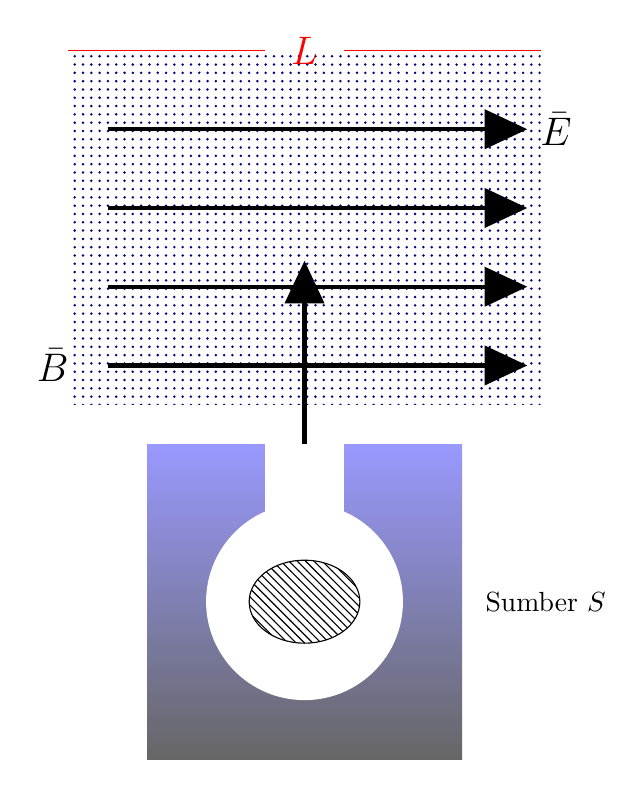
\begin{tikzpicture}
        %GRID
        %\draw[lightgray] (0,0) grid (6,10);
        %KOORDINAT
        \coordinate (L) at (3,2);
        \coordinate (A) at (1,0);
        \coordinate (B) at (5,0);
        \coordinate (C) at (5,4);
        \coordinate (D) at (1,4);
        %POLA
        \fill[pattern=dots, pattern color=blue!50!black] (0,4.5) rectangle (6,9);
        
        %KOTAK%
        \fill [top color=white!60!blue, bottom color=white!40!black] (A) -- (B) -- node [right=5pt]{Sumber $S$}(C) -- (D) -- cycle;
        %LINGKARAN
        \fill[white] (3,2) circle (1.25cm);
        \fill[white] (2.5,2.5) rectangle (3.5,4.25);
        \draw[pattern=north west lines] (3,2) ellipse (20pt and 15pt);
        %PANAH
        \draw[ultra thick] (3,4) -- (3,6) node[currarrow, pos=1, xscale=1, sloped, scale=3]{};

        \draw[ultra thick](0.5,5)  node [left=10pt]{\Large $\bar{B}$} -- (5.5,5) node[currarrow, pos=1, xscale=1, sloped, scale=3]{};
        \draw[ultra thick] (0.5,6) -- (5.5,6) node[currarrow, pos=1, xscale=1, sloped, scale=3]{};
        \draw[ultra thick] (0.5,7) -- (5.5,7) node[currarrow, pos=1, xscale=1, sloped, scale=3]{};
        \draw[ultra thick] (0.5,8) -- (5.5,8) node[currarrow, pos=1, xscale=1, sloped, scale=3]{} node [right=10pt]{\Large $\bar{E}$};

        \draw[red] (0,9) -- (6,9);
        \draw[white] (2.5,9) -- (3.5,9) node [midway, red] {\Large $L$};

    \end{tikzpicture}
\end{center}
    \begin{enumerate}
        \item $\frac{1}{2}mE^2B^2$.
        \item $\frac{1}{2}m\frac{E^2}{B^2}$.
        \item $\frac{1}{2}m\frac{B^2}{E^2}$.
        \item $\frac{1}{2}m\frac{E}{B}$.
        \item $\frac{1}{2}m\frac{B}{E}$.
    \end{enumerate}
  
%17%
\item Unsur helium pertama kali diketahui berada di matahari.
    \begin{enumerate}
        \item Fakta itu diperoleh dengan analisis kimiawi terhadap sampel yang diambil dari matahari.
        \item Fakta itu diketahui dari analisis fotosintesis.
        \item Fakta itu diperoleh dari fosil yang ada di bumi.
        \item Fakta itu diketahui dari spektrum radiasi matahari.
        \item Fakta itu diketahui dari gravitasi matahari.
    \end{enumerate}
     
%18%
\item Sebuah kelereng (massa $m$) tergantung di ujung bawah tali (tanpa massa) dengan panjang $L$. Kelereng tersebut mengalami gerak melingkar beraturan (jari-jari $r$) dengan kecepatan sudut tetap $\omega$. Besar gaya tegangan tali adalah\dots
\begin{center}
    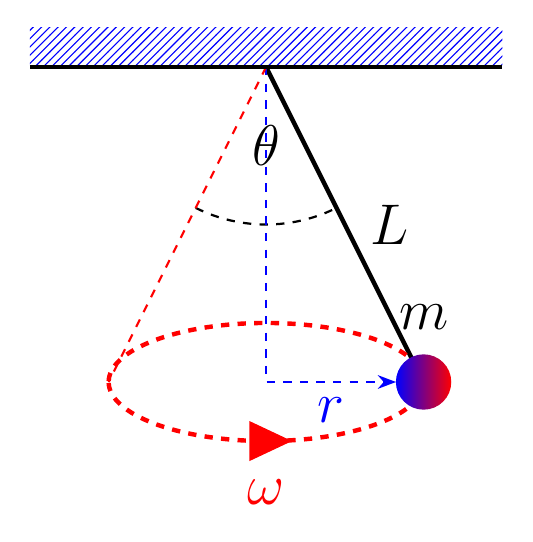
\begin{tikzpicture}
        %GRID
        %\draw[lightgray] (0,0) grid (6,5);
        %KERUCUT
        \coordinate (A) at (5,1);
        \coordinate (B) at (3,5);
        \coordinate (C) at (1,1);
        \tkzMarkAngle[size=2,dashed,thick](C,B,A);
        \tkzLabelAngle (C,B,A){\huge $\theta$};
        \draw[ultra thick] (3,5) --node[midway, right=5pt]{\huge $L$} (5,1)  node [right=5pt, above=15pt]{\huge $m$};
        \draw[ultra thick, dashed, red] (5,1) arc (0:180:2 and 0.75);
        \draw[ultra thick, white] (5,1) arc (0:-180:2 and 0.75) node[currarrow, sloped, pos=0.5, scale=3, xscale=1, color=red]{};
        \draw[ultra thick, dashed, red] (5,1) arc (0:-180:2 and 0.75) node[midway, below=10pt]{\huge $\omega$};
        \draw[dashed, blue, -Stealth, thick] (3,5) -- (3,1) -- (4.65,1) node[midway, below=2pt]{\huge $r$};
        \draw[thick, red, dashed] (3,5) -- (1,1);
        \shade[right color=red, left color=blue] (5,1) circle (10pt);
        %ATAP
        \fill[pattern=north east lines, pattern color=blue] (0,5) rectangle (6,5.5);
        \draw[ultra thick] (0,5) -- (6,5);
    \end{tikzpicture}
\end{center}
    \begin{enumerate}
        \item $m\sqrt{\omega^4r^2+g^2}$
        \item $m\sqrt{\omega^2r^2+g^2}$
        \item $mg \cos{\left(\frac{\theta}{2} \right)}$
        \item $\frac{mgr}{L}$
        \item $\frac{m\omega r}{\sin{\left(\frac{\theta}{2} \right)}}$
    \end{enumerate}
   
%19% 
\item Sebuah planet yang berbentuk bola memiliki rapat massa rata-rata dua kali rapat massa rata-rata bumi, sedangkan jari-jarinya hanya setengah jari-jari bumi. Jika sebuah benda di permukaan bumi memiliki berat $100 \; N$, maka berat benda di permukaan planet tersebut adalah\dots
    \begin{enumerate}
        \item $400 \; N$
        \item $200 \; N$
        \item $100 \; N$
        \item $50 \; N$
        \item $25 \; N$
    \end{enumerate}

%20%
\item Anda dapat melihat dan membaca tulisan pada  kertas soal ini karena kertasnya\dots
    \begin{enumerate}
        \item Mempolarisasi cahaya
        \item Membiaskan cahaya
        \item Menyerap cahaya
        \item Memantulkan cahaya
        \item Memancarkan cahaya
    \end{enumerate}

%21%
\item Sangkar $S$ bermassa $10 \; kg$ berisi benda $B$ bermassa $40 \; kg$, ditarik dengan tali vertikal ke atas oleh gaya sebesar $600 \; N$ seperti pada gambar. Besar gaya normal yang dialami benda dari dasar sangkar
adalah\dots \\
\textbf{($g=10 \; m/s^2$)}
\begin{center}
    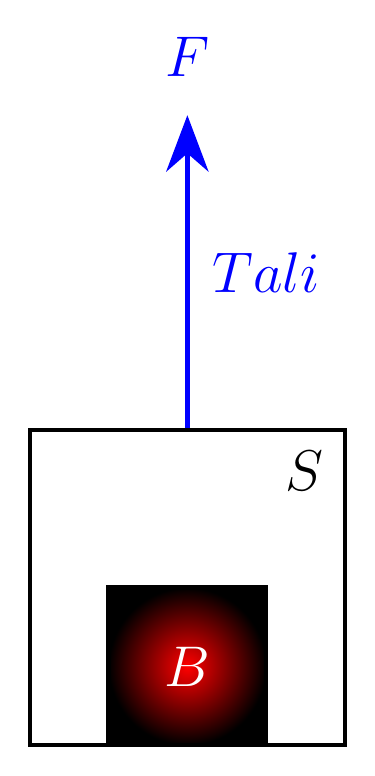
\begin{tikzpicture}
        %GRID
        %\draw[lightgray] (0,0) grid (6,10);
        %TALI
        \draw[ultra thick, -{Stealth[scale=2]}, blue] (3,4) --node[right=5pt]{\huge $Tali$} (3,8) node[above=10pt] {\huge ${F}$}; 
        %BENDA
        \shade[inner color=red, outer color=black] (2,0) rectangle (4,2);
        \draw[ultra thick] (2,0) rectangle (4,2) node [midway, white] {\huge $B$};
        %SANGKAR
        \draw[ultra thick] (1,0) rectangle (5,4) node [below left=5pt]{\huge $S$};
    \end{tikzpicture}
\end{center}

    \begin{enumerate}
        \item $600 \; N$
        \item $480 \; N$
        \item $400 \; N$
        \item $320 \; N$
        \item $300 \; N$
    \end{enumerate}
    
%22% 
\item Sebuah peralatan memiliki taraf intesitas bunyi rata-rata $75 \; dB$. Jika terdapat sejumlah peralatan yang sama dinyalakan, maka taraf intensitas bunyinya menjadi $95 \; dB$. Jumlah peralatan tersebut adalah\dots
    \begin{enumerate}
        \item $10$
        \item $50$
        \item $75$
        \item $100$
        \item $1000$
    \end{enumerate}
    
%23%
\item Seutas kawat penghantar yang dibentuk menjadi bangun seperti pada gambar. Sisi-sisi bangun itu panjangnya $I$. Kawat itu dialiri arus listrik dengan kuat arus $i$ dan diletakkan dalam medan magnet yang berarah masuk bidang gambar secara tegak lurus. Jika besar induksi magnetnya $B$, maka tentukan besar gaya magnet total yang dialamai oleh kawat itu.
\begin{center}
    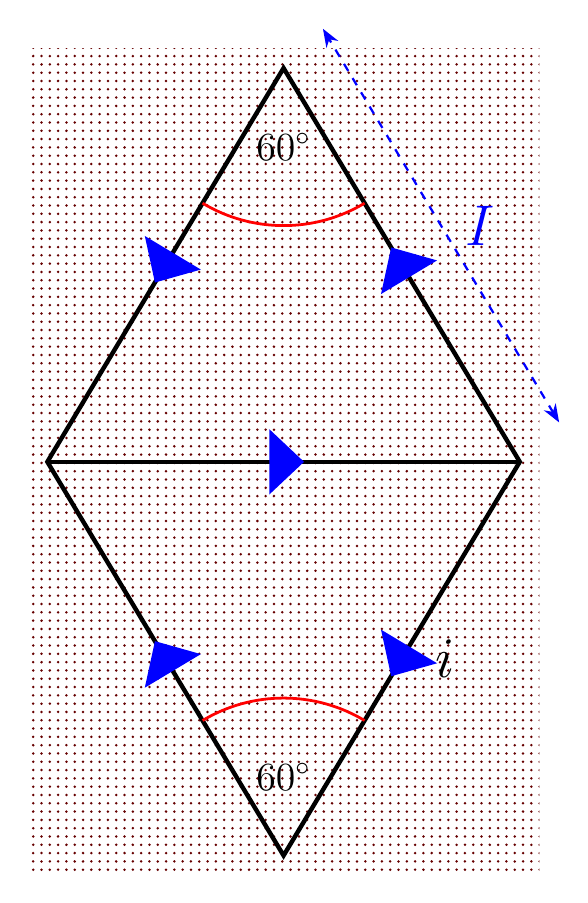
\begin{tikzpicture}
        %GRID
        %\draw[blue] (0,0) grid (10,11);
        %POLA
        \fill[pattern=dots,pattern color=red!40!black] (-0.25,-0.25) rectangle (6.25,10.25);
        %KOORDINAT
        \coordinate (A) at (3,0);
        \coordinate (B) at (6,5);
        \coordinate (C) at (3,10);
        \coordinate (D) at (0,5);
        %GARIS
        \draw[ultra thick] (A) -- node [currarrow, sloped, scale=5, pos=0.5, xscale=-0.5, color=blue] {} (B)  node[midway, right=8pt]{\huge $i$} -- node [currarrow, sloped, scale=5, pos=0.5, xscale=-0.5, color=blue] {} (C) -- node [currarrow, sloped, scale=5, pos=0.5, xscale=-0.5, color=blue] {} (D) -- node [currarrow, sloped, scale=5, pos=0.5, xscale=-0.5, color=blue] {} cycle;
        \draw[ultra thick] (B) -- node [currarrow, sloped, scale=5, pos=0.5, xscale=0.5, color=blue] {} (D);
        %SUDUT
        \tkzMarkAngle[line width=1pt, color=red, size=2](B,A,D);
        \tkzLabelAngle (B,A,D) {\Large $60^\circ$};
        
        \tkzMarkAngle[line width=1pt, color=red, size=2](D,C,B);
        \tkzLabelAngle (D,C,B) {\Large $60^\circ$};
        %GARIS BANTU
        \draw[thick, dashed, color=blue, Stealth-Stealth] (6.5,5.5) -- (3.5,10.5) node [midway, right=5pt] {\huge $I$};
    \end{tikzpicture}
\end{center}
    \begin{enumerate}
        \item $iIB$
        \item $2iIB$
        \item $3iIB$
        \item $4iIB$
        \item $5iIB$
    \end{enumerate}
    
%24%  
\item Sebuah pesawat yang bergerak meninggalkan bumi menembakkan peluru dengan arah yang sama dengan arah pesawat. Jika kecepatan peluru terhadap bumi dan pesawat
masing-masing adalah $0,75c$ dan $0,4c$, maka kecepatan pesawat terhadap bumi adalah\dots \\
\textbf{($c=$ laju cahaya)}
	\begin{enumerate}
		\item $0,35c$
		\item $0,4c$
		\item $0,5c$
		\item $0,6c$
		\item $0,64c$
	\end{enumerate}
	
%25%
\item Ditinjau pencampuran dua macam sampel zat cair sejenis tapi berbeda suhunya. Massa sampel yang lebih panas $m_1$, sama dengan dua kali massa sampel yang lebih dingin $m_2$. Suhu awal sampel yang lebih panas $T_1$, sama dengan dua kali suhu awal sampel yang lebih dingin
$T_2 = 30^\circ \; C$. Suhu campuran pada keadaan setimbang adalah\dots
   \begin{enumerate}
        \item $55^\circ \; C$
        \item $50^\circ \; C$
        \item $45^\circ \; C$
        \item $40^\circ \; C$
        \item $35^\circ \; C$
   \end{enumerate}
   
%beginrandom%
   
%26%
\item Sebuah gaya konstan bekerja pada suatu massa $m_1$. Kemudian massa $m_2$ ditarnbahkan pada massa tadi sehingga percepatan sistem berkurang menjadi $\frac{1}{5}$ kali percepatan semula. Dengan menganggap gaya yang bekerja tidak berubah, maka nilai perbandingan $\frac{m_1}{m_2}$ adalah\dots
    \begin{enumerate}
        \item $1$
        \item $\frac{1}{2}$
        \item $\frac{1}{3}$
        \item $\frac{1}{4}$
        \item $\frac{1}{5}$
    \end{enumerate}
  
%27%  
\item Sebuah batu dilemparkan dari tanah vertikal ke atas dengan kecepatan awal $v_0=\sqrt{7} \; m/s$. Ketika sampai pada ketinggian $h$, kecepatannya menjadi $v$, sedangkan ketika ketinggiannya dua kalinya, kecepatannya menjadi
setengahnya. Jika $g=10 \; m/s^2$, nilai $h$ adalah\dots
    \begin{enumerate}
        \item $\frac{1}{20} \; m$
        \item $\frac{1}{10} \; m$
        \item $\frac{3}{20} \; m$
        \item $\frac{1}{5} \; m$
        \item $\frac{1}{4} \; m$
    \end{enumerate}
    
%28%  
\item Selang yang terbuat dari bahan elastik memiliki panjang $l \; m$. Jari-jari rongga selang itu $1 \; cm$. Tetapan elastik silinder itu $0,6 \; N/m$. Selang itu diisi sepenuhnya dengan bahan elastik lain yang bermodulus Young $2000 \; N/m^2$. Tentukan tetapan elastik selang dan isinya.
    \begin{enumerate}
        \item $0,307 \; N/m$
        \item $0,628 \; N/m$
        \item $1,228 \; N/m$
        \item $1,536 \; N/m$
        \item $1,812 \; N/m$
    \end{enumerate}

%29%  
\item Sumber bunyi mendekati pendengar yang diam dengan kecepatan $v_s$. Ketika sumber memancarkan bunyi dengan
frekuensi $400 \; Hz$, pendengar mendengar bunyi tersebut dengan frekuensi $500 \; Hz$. Apabila kecepatan bunyi di udara adalah $v$, maka nilai $\frac{v_s}{v}$ adalah\dots
    \begin{enumerate}
        \item $\frac{1}{5}$
        \item $\frac{1}{4}$
        \item $\frac{4}{5}$
        \item $\frac{6}{5}$
        \item $\frac{5}{4}$
    \end{enumerate}

%30%
\item Seutas kawat tembaga menembus permukaan meja secara vertikal (lihat gambar). Kawat itu dialiri arus listrik searah ke atas. Ruang diatas meja tersebut berisi medan magnet luar seragam berarah ke bawah. Sebuah partikel mula-mula berada pada sebuah titik diatas meja dengan jarak $R$ dari kawat. Partikel bermuatan $q$ itu diberi kecepatan $\bar{v_0}$ yang arahnya tegak lurus terhadap garis penghubung titik tempat partikel itu mula-mula ke kawat berarus. Jika massa pertkel itu $m$, medan magnet luar $\bar{B}$ dan besar arus $i$, berapakah kecepatan awal $\bar{v_0}$ agar partikel itu bergerak melingkar?
\begin{center}
    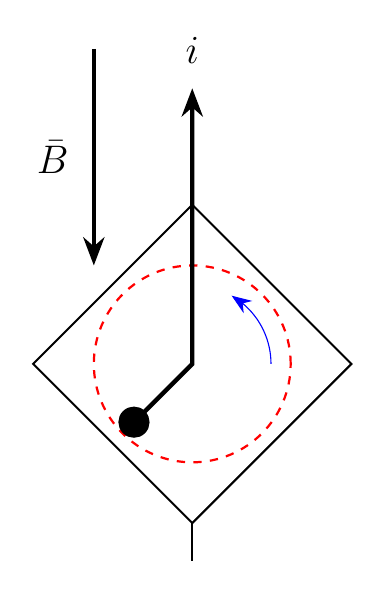
\begin{tikzpicture}
        %GRID
        %\draw[lightgray] (0,0) grid (7,7);
        %KOORDINAT
        \coordinate (A) at (3,0);
        \coordinate (B) at (5,2);
        \coordinate (C) at (3,4);
        \coordinate (D) at (1,2);
        \coordinate (L) at (3,2);
        %KOTAK
        \draw[thick] (3,0) -- (3,-0.5);
        \draw[ultra thick] (A) -- (B) -- (C) -- (D) -- cycle;
        \fill[fill=white] (A) -- (B) -- (C) -- (D) -- cycle;
        %LINGKARAN
        \draw[dashed, color=red, thick] (L) circle (1.25cm);
         %GARIS PANAH ATAS
        \draw[ultra thick, {Circle[scale=1.5]}-Stealth] (2.12,1.12) -- (L) -- (3,5.5) node[above=5pt]{\Large $i$};
        %PANAH IN LINGKARAN
        \draw[blue, -{Stealth[scale=1.5]}] (4,2) arc (0:60:1cm and 1cm);
        %PANAH KE BAWAH
        \draw[ultra thick, -Stealth] (1.75,6) -- (1.75,3.25) node [midway, left=5pt]{\Large $\bar{B}$};
    \end{tikzpicture}
\end{center}
    \begin{enumerate}
        \item $2\frac{Bi}{mR}$
        \item $\frac{qBm}{R^2}$
        \item $\frac{2qBR}{m}$
        \item $\frac{qBR}{m}$
        \item $\frac{2 \pi qBR}{m}$
    \end{enumerate}
 
%31%
\item Selama $120$ hari intensitas radiasi bahan radioaktif berkurang tinggal $\frac{1}{8}$ intensitas mula-mula. Umur paruh bahan radioaktif tersebut adalah\dots
    \begin{enumerate}
        \item $60$ hari
        \item $50$ hari
        \item $40$ hari
        \item $30$ hari
        \item $15$ hari
    \end{enumerate}

%32%
\item Dua planet $A$ dan $B$ masing-masing pada lintasan berbentuk eJips. Perbandingan periodenya $\frac{T_A}{T_B}=8$. Nilai perbandingan setengah sumbu panjang lintasannya $\frac{a_A}{a_B}$, adalah\dots
    \begin{enumerate}
        \item $16$
        \item $12$
        \item $6$
        \item $4$
        \item $2$
    \end{enumerate}

%endrandom%

%33%
\item Rangkaian resistor-induktor-kapasitor disusun seri dengan resistansi $R=400 \; \Omega$, reaktansi induktif $X_L=500 \; \Omega$ dari impedansi rangkaian $Z = 500 \; \Omega$. Berapa nilai reaktansi kapasitif dari kapasitor?
    \begin{enumerate}
        \item $200 \; \Omega$
        \item $300 \; \Omega$
        \item $400 \; \Omega$
        \item $500 \; \Omega$
        \item $600 \; \Omega$
    \end{enumerate}

%34%
\item Dua sistem getaran selaras sederhana identik $A$ dan $B$, masing-masing berupa massa $m$ terikat pada pegas dengan tetapan gaya $k$. Apabila amplitudo $B \; 40 \; cm$
amplitudo $A \; 20 \; cm$, nilai perbandingan kecepatan kedua getaran pada saat simpangan keduanya sama, $10 \; cm$ adalah $\frac{v_B}{v_A}=$\dots
    \begin{enumerate}
        \item $\sqrt{2}$
        \item $\sqrt{3}$
        \item $2$
        \item $\sqrt{5}$
        \item $\sqrt{6}$
    \end{enumerate}

%35%
\item Termometer $X$ menunjukkan angka $-20^\circ$ pada titik beku air $130^\circ$ pada titik didih air. Suhu $X$ dan Celsius akan menunjukkan angka yang sama pada\dots
    \begin{enumerate}
        \item $60^\circ$
        \item $45^\circ$
        \item $40^\circ$
        \item $30^\circ$
        \item $20^\circ$
    \end{enumerate}

\end{enumerate}
\end{document}  
